В ходе обсуждения архитектуры рекомендательной системы, было принято решение по
ее реализации в виде микро-сервиса. Модель взаимодействия подсистем можно увидеть
на изображении ниже.
\begin{figure}[H]
  \centering
  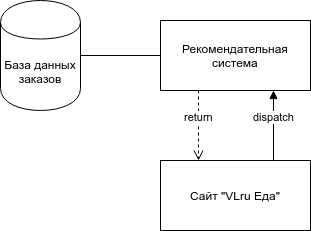
\includegraphics[scale=0.8]{images/sub_modules.png}
  \caption{Взаимодействие всех систем}
\end{figure}
На данный момент в компании активно внедряется такая технология, как Kubernetes.
В результате настойки непрерывного интегрирования и развертывания, процесс
разработки и обновления представлен на изображении \ref{deploy}.
\begin{figure}[H]
  \label{deploy}
  \centering
  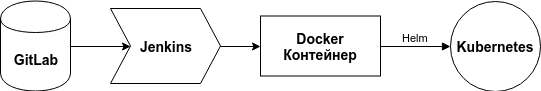
\includegraphics[scale=0.8]{images/deploy.png}
  \caption{Процесс развертывания}
\end{figure}
После написания кода, разработчик запускает \textit{Job} (задачу) в Jenkins, который
собирает Docker контейнер. Когда необходимо развернуть сборку на сервере, запускается
другая задача, которая при помощи Helm доставляет контейнер в Kubernetes. Таким
образом достигается:
\begin{enumerate}
  \item Отказоустойчивость, т.к. в кластере Kubernetes одновременно работают
  3 репликации приложения
  \item Постоянная работа микро-сервиса, т.к. во время обновления реплики обновляются
  один за другим
\end{enumerate}
